\documentclass{beamer}
\DeclareFontShape{OT1}{cmss}{b}{n}{<->ssub * cmss/bx/n}{} 
\usetheme{default}
\usepackage{amsmath}
\usepackage{amsfonts}
\usepackage{mathbbol}
\usepackage{xcolor} % before tikz or tkz-euclide if necessary
\usepackage{tkz-euclide} % no need to load TikZ
\usepackage{multirow}
\usepackage{lmodern}
\usepackage{bm}
\usepackage{hyperref}
\usepackage{subfigure}

\titlegraphic{
\includegraphics[width=2cm]{../../Figures/UAMS_RGB.png}
}


\title{Single-Cell RNA-seq Analysis\\ Methods Overview}
\author{Horacio G\'omez-Acevedo\\ Department of Biomedical Informatics\\
	University of Arkansas for Medical Sciences}
\begin{document}
	\begin{frame}[plain]
		\maketitle
	\end{frame}
	\begin{frame}{sc-RNA seq}
		
\begin{figure}[h]
	\centering
	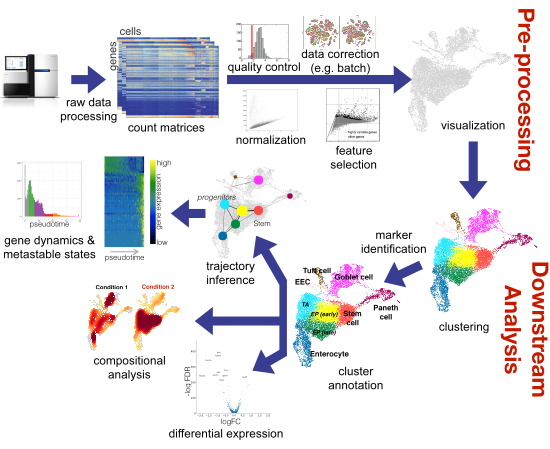
\includegraphics[scale=0.25]{../../Figures/scrnaseq_overview.png}
	\caption{\href{https://github.com/theislab/single-cell-tutorial}{Overview}}
\end{figure}
\end{frame}

\begin{frame}{Bulk vs Single-cell RNAseq}
	
\begin{figure}%
	\centering
	\subfigure[ Bulk RNAseq]{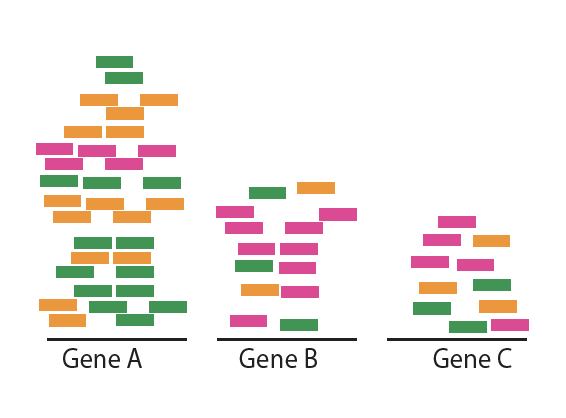
\includegraphics[scale=0.4]{../../Figures/bulk_rnaseq.png} }%
	\qquad
	\subfigure[ Sc-RNAseq]{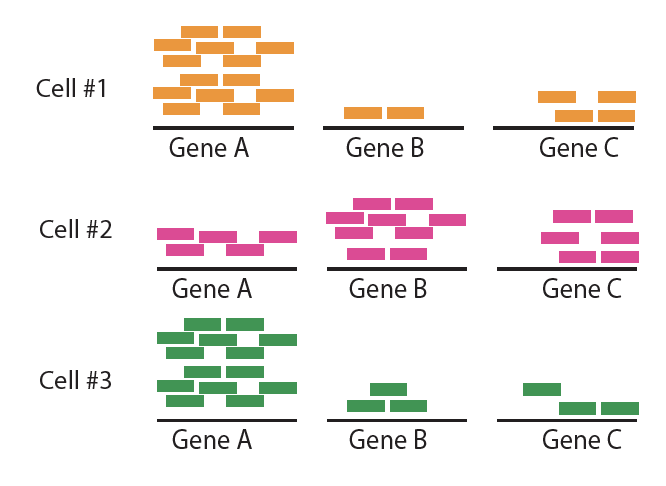
\includegraphics[scale=0.4]{../../Figures/sc_rnaseq.png} }%
%	\caption{2 Figures side by side}%
%	\label{fig:example}%
\end{figure}
	
\end{frame}

	
	\begin{frame}{Space: the final frontier}
		
The mathematical representation of the data is given by placing the readings (RPKM) of each individual gene in an "axis" of an $n$ dimensional space.
 In this case $n$ represents a large number of genes.
 
\begin{figure}[h]
	\centering
	\includegraphics[scale=0.45]{../../Figures/sc_space.png}
	\caption{Spatial representation of scRNAseq data}
\end{figure}
		
	\end{frame}
	
\begin{frame}{PCA interlude}

Principal Component Analysis is one of the most commonly used methodologies to "inspect" high dimensional data. 

\begin{figure}[h]
	\centering
	\includegraphics[scale=0.45]{../../Figures/sc_space1.png}
	\caption{Plane projection of data}
\end{figure}	
	
\end{frame}	

\begin{frame}{PCA projection}
	The main goal of PCA  is to find the representation of our data in a lower dimensional space (mostly a plane). But the selection of such plane should preserve original data variability. 
	
	Formally, the two directions represent the directions of the maximal variability of our data. 

\end{frame}	

\begin{frame}{RGB example}
\begin{figure}[h]
	\centering
	\includegraphics[scale=0.45]{../../Figures/pca_rgb.png}
	\caption{Plane projection of RGB data}
\end{figure}		


\end{frame}	

\begin{frame}{Clustering}
	Clustering refers to a set of computational techniques for finding subsets or {\sl clusters} in a data set.  Clustering is among the so-called {\bf unsupervised learning methodologies } .\\
	
	\begin{center}
		Unsupervised $\ne$ Automatic
	\end{center}
	
	Thus, the main goal of clustering is to find homogeneous subgroups among the data. 
		
\end{frame}
	
\begin{frame}{Clustering terminology}
	


Let's define a distance between two points (in a plane), say $d$. Also, the {\sl centroid } of a cluster is the mean of their observations.

\begin{figure}[h]
	\centering
	\includegraphics[scale=0.65]{../../Figures/centroid.png}
	\caption{Distance and Centroid of a cluster}
\end{figure}	
\end{frame}

\begin{frame}{K-means clustering}
One of the simplest methods for clustering is $K$-means clustering. 

We begin with a data set and a value $K$ fixed by a human (say $K=3$). 

\begin{enumerate}
	\item Assign randomly a value between 1 and K to each data point.
	\item Iterate the following procedure until the clusters assignments stop changing 
	\begin{enumerate}
		\item Find the centroid for each of the $K$ clusters.
		\item Each point will be assigned to the cluster $K$ whose distance is the smallest. If two or more are equidistant, select randomly the cluster among the equidistant clusters.
	\end{enumerate}	
\end{enumerate}


\end{frame}

\begin{frame}{K-means clustering picture}
	
	\begin{figure}[h]
		\centering
		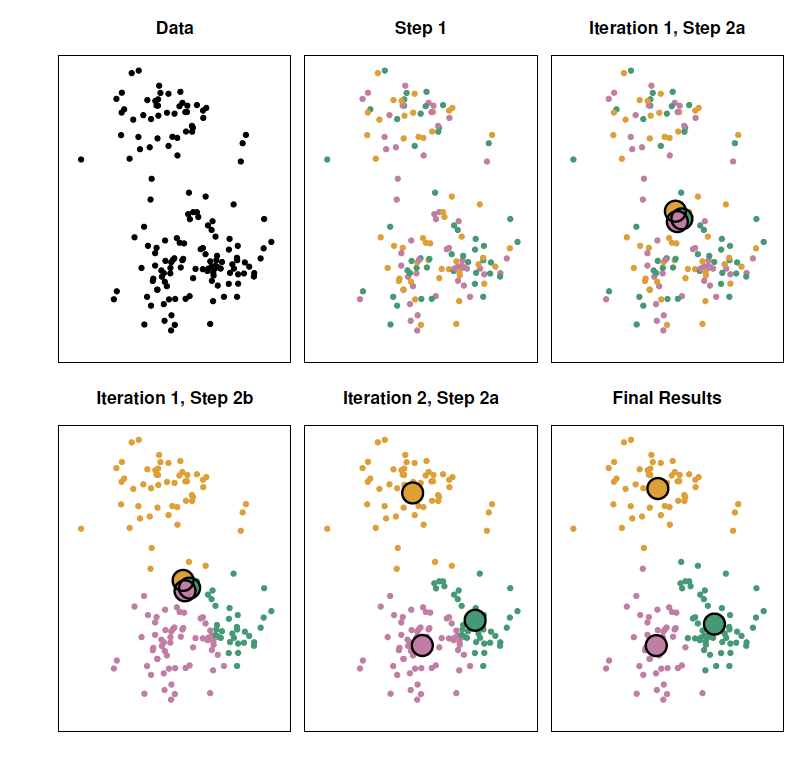
\includegraphics[scale=0.55]{../../Figures/kmeans_clustering.png}
		%\caption{Distance and Centroid of a cluster}
	\end{figure}	
	\href{https://www.statlearning.com/}{An Introduction to Statistical Learning (Chapter 10)}
\end{frame}

\begin{frame}{Problems with K-means clustering}
	\begin{itemize}

		\item Selection of the distance function $d$ (Euclidean, Pearson correlation, arccos, etc.) 
		\item Selection of $K$.
	\end{itemize}
	\begin{figure}[h]
	\centering
	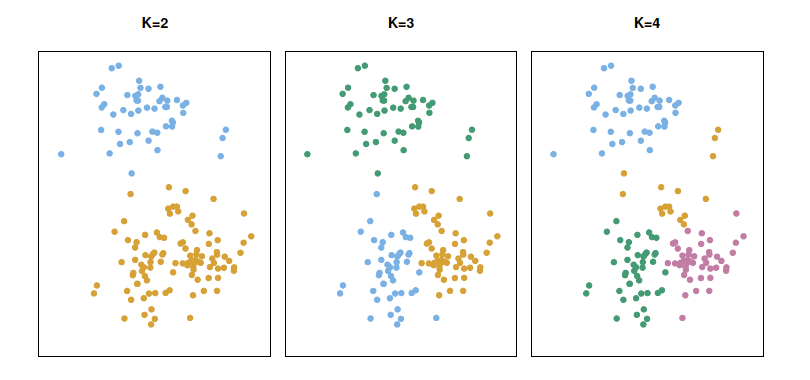
\includegraphics[scale=0.55]{../../Figures/kmeans_K.png}
	%\caption{Distance and Centroid of a cluster}
\end{figure}	
\href{https://www.statlearning.com/}{An Introduction to Statistical Learning (Chapter 10)}	
	
\end{frame}
	
\begin{frame}{t Stochastic Neighbor Embedding}

$t$-SNE maps a set of high-dimensional points to a plane, such that ideally, close neighbors remain close and distant points remain distant.

 Informally, the algorithm places all
points on the 2D plane, initially at random positions, and lets them
interact as if they were physical particles. 

The interaction is governed
by two laws: 
\begin{itemize} 
	\item all points are repelled from each other
\item each point is attracted to its nearest neighbors
\end{itemize}
This methodology is governed by a parameter called {\bf perplexity}.

\end{frame}	

\begin{frame}{tSNE vs PCA}
	
		\begin{figure}[h]
		\centering
		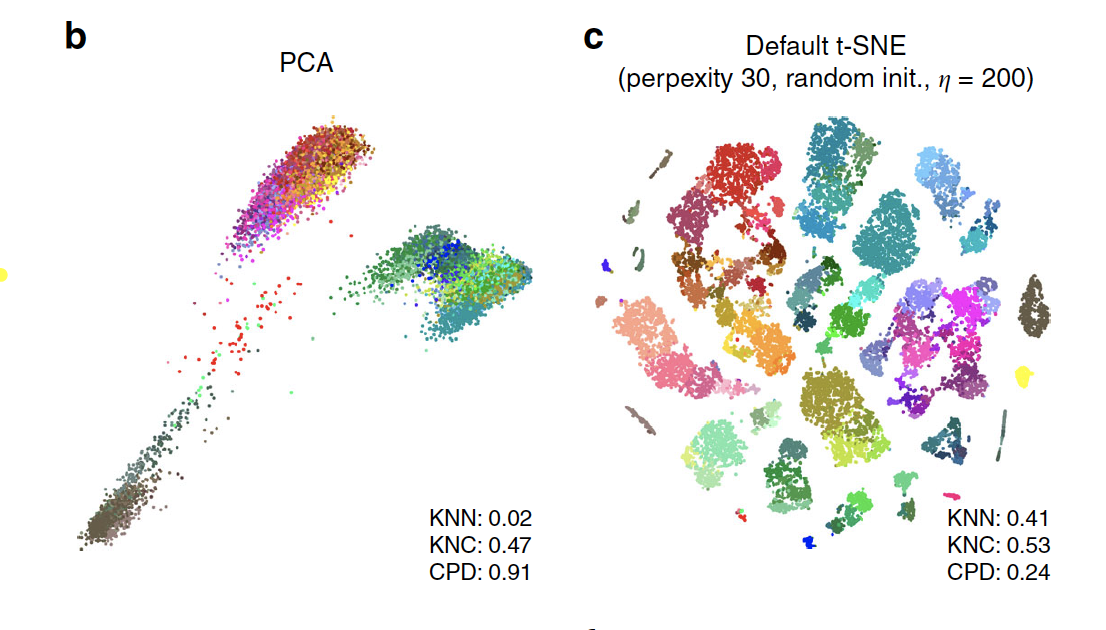
\includegraphics[scale=0.55]{../../Figures/pca_vs_tsne.png}
		\caption{\href{https://doi.org/10.1038/s41467-019-13056-x}{A Visual Comparison of PCA and tSNE}}
	\end{figure}	
	
	
\end{frame}
	
\begin{frame}{Community Detection}
	We can also add another layer of complexity to our clustered 2d data by using {\bf graphs}.
		\begin{figure}[h]
	\centering
	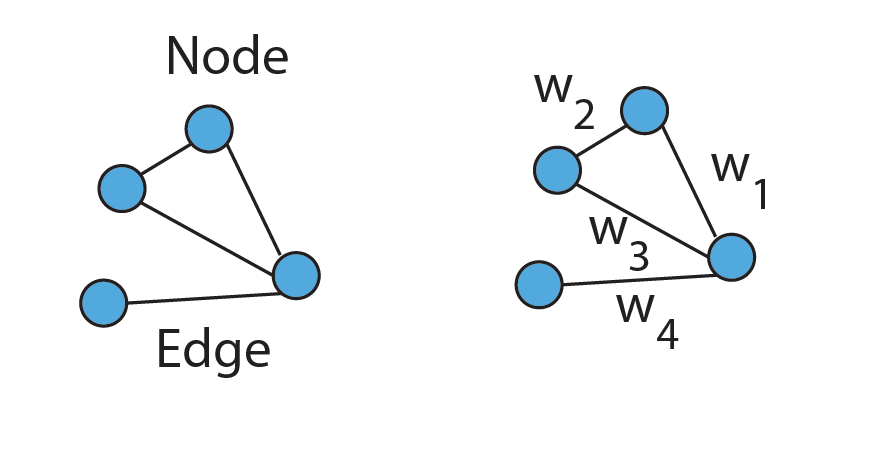
\includegraphics[scale=0.45]{../../Figures/graph_notation.png}
%	\caption{\href{https://doi.org/10.1038/s41467-019-13056-x}{A Visual Comparison of PCA and tSNE}}	
\end{figure}
	 
\end{frame}
	
\begin{frame}{MST clustering}
	A tree is a graph that when adding an edge will form a cycle.
	A minimum spanning tree (MST) of a weighted graph is the minimum weight set or edges that connects all the vertices. 
	
			\begin{figure}[h]
		\centering
		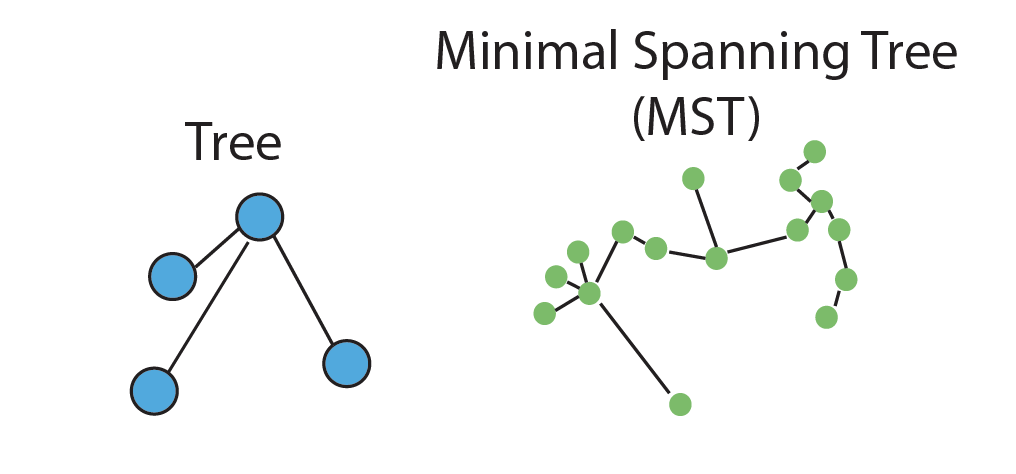
\includegraphics[scale=0.45]{../../Figures/tree_mst.png}
		%	\caption{\href{https://doi.org/10.1038/s41467-019-13056-x}{A Visual Comparison of PCA and tSNE}}	
	\end{figure}	
\end{frame}	

\begin{frame}{Clustering via MST}
	
	The advantage to use graph algorithms is speed which is more evident as the number of interactions increases. 
	
	Also, graphs are very intuitive as it is shown with the clustering using MST. Namely, deleting the longest $K$ edges, we can cluster the data ($K=3$ for the graph on the right) 
	
				\begin{figure}[h]
		\centering
		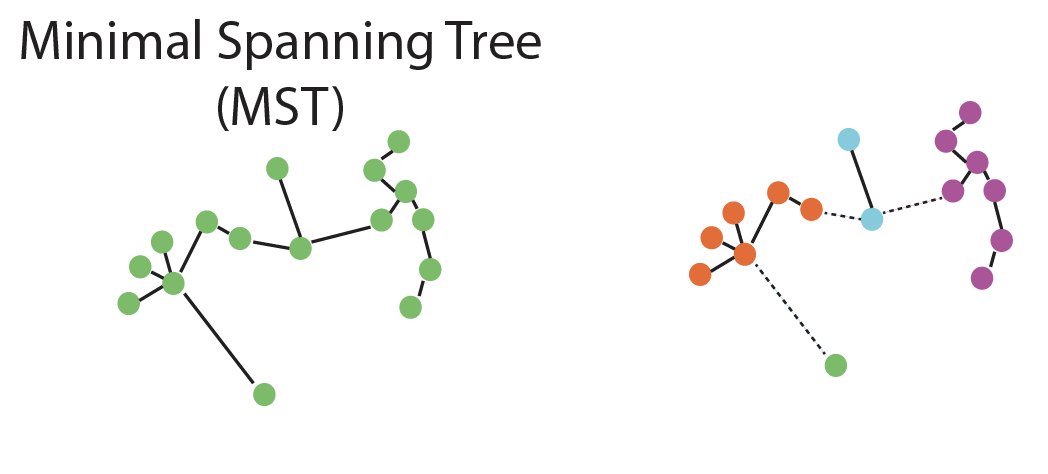
\includegraphics[scale=0.45]{../../Figures/mst_clustering.png}
		%	\caption{\href{https://doi.org/10.1038/s41467-019-13056-x}{A Visual Comparison of PCA and tSNE}}	
	\end{figure}	
	
	
	
\end{frame}

\begin{frame}{KNN graph}
	The K-nearest neighbors (KNN) graph is a graph which two vertices $p$ and $q$ are connected by an edge if the distance between $p$ and $q$ are among the $K$th smallest distances.
	
	A word of caution. KNN is a method commonly for classification. This means that we already know something about our data and we will classify an unknown sample. It is not the same as KNN graph.
	
	
\end{frame}

\begin{frame}{Chameleon}
	An important graphic method for clustering is called \href{https://doi.org/10.1109/2.781637}{Chameleon}

				\begin{figure}[h]
	\centering
	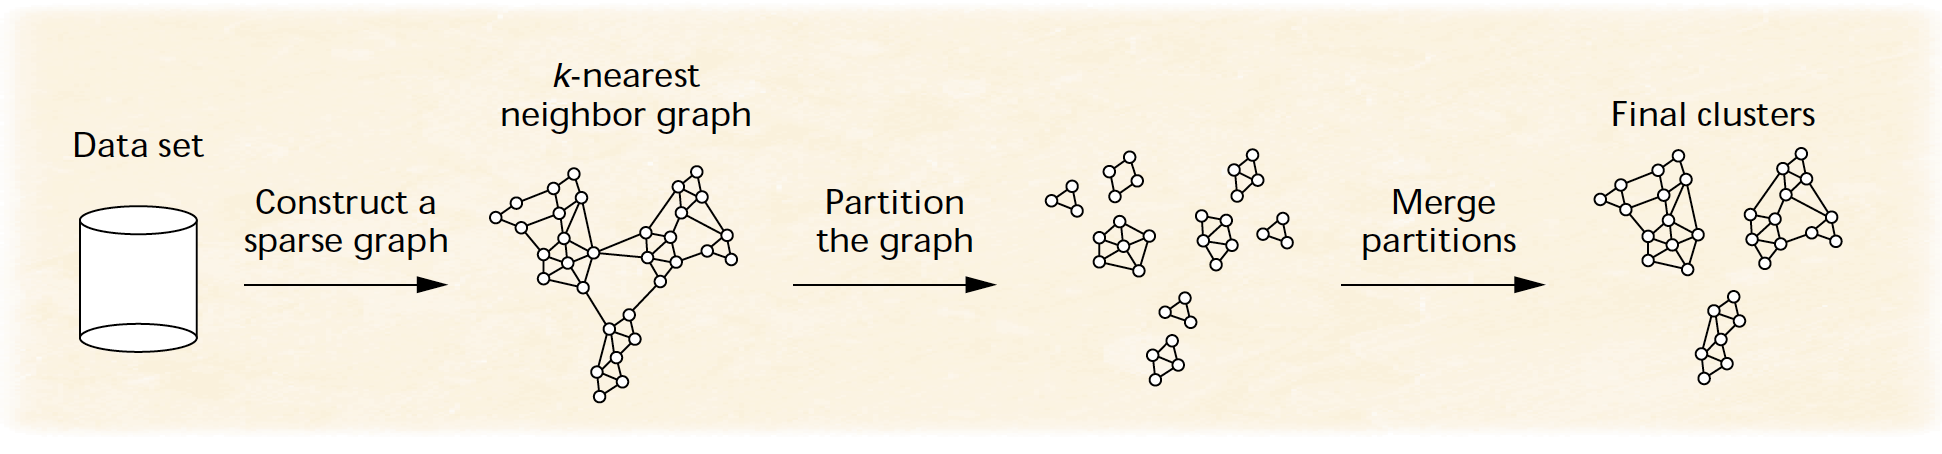
\includegraphics[scale=0.3]{../../Figures/chameleon.png}
	%	\caption{\href{https://doi.org/10.1038/s41467-019-13056-x}{A Visual Comparison of PCA and tSNE}}	
\end{figure}	
Chameleon uses a dynamic modeling framework to
determine the similarity between pairs of clusters by looking
at their relative interconnectivity (RI) and relative
closeness (RC).
	
\end{frame}

\begin{frame}{Cluster Annotation}
	Once we have done the clustering, we are ready to give {\bf annotation} . The so-called {\sl marker genes} characterize the clusters.
	 
				\begin{figure}[h]
	\centering
	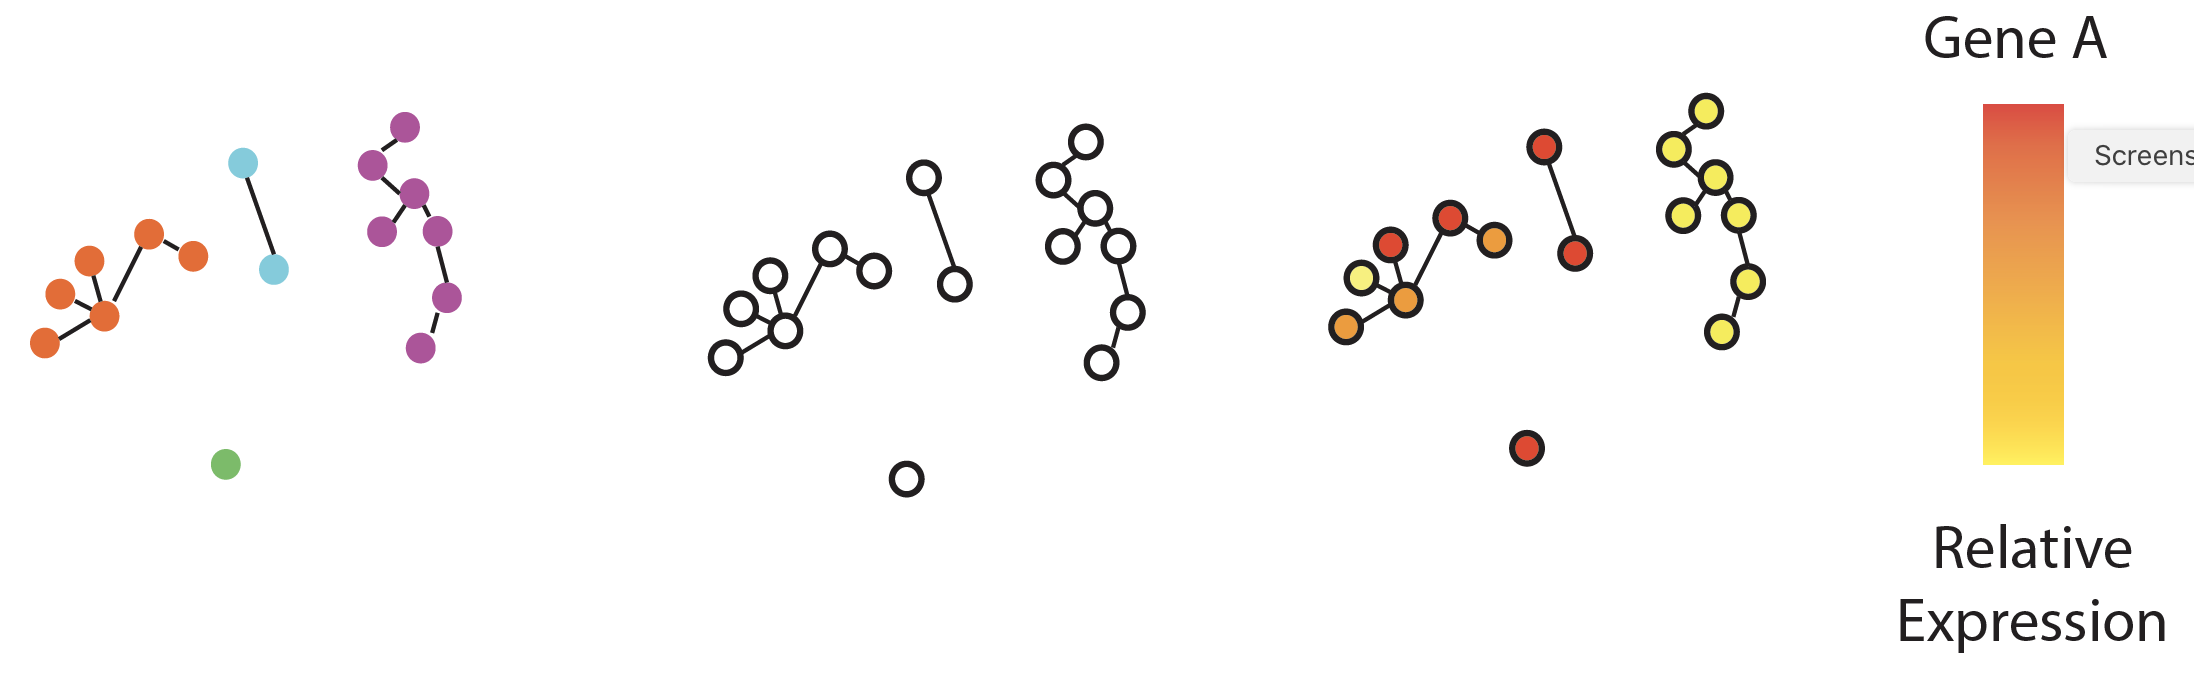
\includegraphics[scale=0.3]{../../Figures/sc_annotation.png}
	%	\caption{\href{https://doi.org/10.1038/s41467-019-13056-x}{A Visual Comparison of PCA and tSNE}}	
\end{figure}		
	
\end{frame}
	
	\begin{frame}{References}
		
		Materials and some of the pictures are from (1). 
		\begin{enumerate}
			\item Gareth James et al. {\it An Introduction to Statistical Learning with applications in R}. Springer (2015)
			\item Robert Sedgewick. {\it Algorithms in C }, 3rd edition. Addison-Wesley (2002) . 
			\item Ke-Lin Du et al. {\it Neural networks and Statistical Learning}, 2nd edition. Springer (2019)
			
		\end{enumerate}	
		
		I have used some of the graphs by hacking TiKz code from StakExchange, Inkscape for more aesthetic plots and other old tricks of \TeX
	\end{frame}	
	
	
\end{document}